% Copyright (c) 2016-2020 The ALF project.
% This is a part of the ALF project documentation.
% The ALF project documentation by the ALF contributors is licensed
% under a Creative Commons Attribution-ShareAlike 4.0 International License.
% For the licensing details of the documentation see license.CCBYSA.

% !TEX root = doc.tex


The ALF  library comes with five model classes: (i) SU(N) Hubbard models, (ii) O(2N) t-V models, (iii) Kondo models, (iv) long-range Coulomb models, and (v) generic $\Ztwo$ lattice gauge theories coupled to $\Ztwo$ matter and fermions. Below we detail the functioning of these classes.  


\subsection{SU(N) Hubbard models \texttt{Hamiltonian\_Hubbard\_mod.F90}} \label{sec:hubbard}

The parameter space for this model class  reads: 

\begin{lstlisting}[style=fortran,escapechar=\#,breaklines=true]
&VAR_Hubbard               !! Variables for the Hubbard class
Mz        = .T.             ! Whether to use the M_z-Hubbard model: Nf=2; N_SUN must be  
                            ! even. HS field couples to the z-component of magnetization
ham_T     = 1.d0            ! Hopping parameter
ham_chem  = 0.d0            ! Chemical potential
ham_U     = 4.d0            ! Hubbard interaction
ham_T2    = 1.d0            ! For bilayer systems
ham_U2    = 4.d0            ! For bilayer systems
ham_Tperp = 1.d0            ! For bilayer systems
/
               
\end{lstlisting}
In the above listing, \texttt{ham\_T} and \texttt{ham\_T2} correspond to the hopping in the first and second layers respectively and  \texttt{ham\_Tperp} is to the interlayer hopping.   The Hubbard $U$ term has an orbital index, \texttt{ham\_U}  for the first and \texttt{ham\_U2} for the second layers.  Finall,  \texttt{ham\_chem}  corresponds to the chemical potential.    If the flag \texttt{Mz} is set to \texttt{.False.}, then the code simulates the following SU(N) symmetric Hubbard model:
\begin{multline}
\hat{H} = \sum_{(\ve{i},\ve{\delta}), (\ve{j},\ve{\delta}')}  \sum_{\sigma =1}^{N}  T_{(\ve{i},\ve{\delta}), (\ve{j},\ve{\delta}')}    \hat{c}^{\dagger}_{(\ve{i},\ve{\delta}), \sigma }   e^{\frac{2 \pi i}{\Phi_0} \int_{\ve{i} + \ve{\delta}}^{\ve{j} + \ve{\delta}'}  
     \vec{A}(\ve{l})  d \ve{l}} \hat{c}^{}_{(\ve{j},\ve{\delta}'),\sigma} \\
 + \sum_{\vec{i}} \sum_{\delta}   \frac{U_{\ve{\delta}} }{N} \left(\sum_{\sigma=1}^{N}  \left[   \hat{c}^{\dagger}_{(\vec{i},\ve{\delta}),\sigma } 
    \hat{c}^{\phantom\dagger}_{(\vec{i}, \ve{\delta}),\sigma }  - 1/2  \right] \right)^2
    - \mu \sum_{(\ve{i},\ve{\delta})}  \sum_{\sigma =1}^{N} \hat{c}^{\dagger}_{(\vec{i},\ve{\delta}),\sigma } \hat{c}^{\phantom\dagger}_{(\vec{i},\ve{\delta}),\sigma } .
\end{multline}
The  generic hopping is taken fron Eq.~\eqref{generic_hopping.eq}   with appropriate boundary conditions given by Eq.~\eqref{generic_boundary.eq}.  The index $\ve{i}$ runs over the unit cells, $\ve{\delta}$ over the orbitals in each unit cell and $\sigma$  from $1$ to $N$  and encodes the SU(N) symmetry.    Note that  $N$ corresponds to \texttt{N\_SUN}  in the code.  The flavor index is set to  unity such that it does not appear in the  Hamiltonian. The chemical potential $\mu$ is relevant only for the finite temperature code. 

If the variable \texttt{Mz} is set to \texttt{.True.}, then the code requires  \texttt{N\_SUN}  to be even and simulates the following Hamiltonian: 
\begin{align}
\hat{H} =& \sum_{(\ve{i},\ve{\delta}), (\ve{j},\ve{\delta}')}  \sum_{\sigma =1}^{N/2}  \sum_{s=1,2} T_{(\ve{i},\ve{\delta}), (\ve{j},\ve{\delta}')}    \hat{c}^{\dagger}_{(\ve{i},\ve{\delta}), \sigma,s }   e^{\frac{2 \pi i}{\Phi_0} \int_{\ve{i} + \ve{\delta}}^{\ve{j} + \ve{\delta}'}  
     \vec{A}(\ve{l})  d \ve{l}} \hat{c}^{}_{(\ve{j},\ve{\delta}'),\sigma,s}     \nonumber   \\
    &- \sum_{\vec{i}} \sum_{\delta}   \frac{U_\delta}{N} \left(\sum_{\sigma=1}^{N/2}  \left[   \hat{c}^{\dagger}_{(\vec{i},\ve{\delta}),\sigma, 2} 
    \hat{c}^{\phantom\dagger}_{(\vec{i}, \ve{\delta}),\sigma,2 }  -  \hat{c}^{\dagger}_{(\vec{i},\ve{\delta}),\sigma, 1} 
    \hat{c}^{\phantom\dagger}_{(\vec{i}, \ve{\delta}),\sigma,1} \right] \right)^2  \nonumber \\
    & - \mu \sum_{(\ve{i},\ve{\delta})}  \sum_{\sigma =1}^{N/2}  \sum_{s=1,2}\hat{c}^{\dagger}_{(\vec{i},\ve{\delta}),\sigma, s} \hat{c}^{\phantom\dagger}_{(\vec{i},\ve{\delta}),\sigma, s}.
\end{align}
In this case, the flavor index \texttt{N\_FL}   takes the value 2. Cleary at $N=2$, both modes  correspond  to the Hubbard model.  For $N$  even and $N > 2$  the models differ.  In particular  in the latter  Hamiltonian the U(N) symmetry is broken down to  U(N/2) $\otimes$ U(N/2).  

Since this model class  works for all predefined lattices  (see Fig.~\ref{fig_predefined_lattices}) 
it includes the SU(N) periodic Anderson model on the square and Honeycomb lattices.
Finally, we note that the executable for this class is given by \texttt{Hubbard.out}.

As an example,  we can consider the periodic Anderson model.   Here we choose  the \texttt{Bilayer\_square}  lattice \texttt{Ham\_U} =  \texttt{Ham\_T2} $= 0$,  \texttt{Ham\_U2}$=U_f$,  \texttt{Ham\_tperp}$=V$  and \texttt{Ham\_T}$=1$.   The  pyALF  based python script    \href{https://git.physik.uni-wuerzburg.de/ALF/pyALF/-/blob/master/Scripts/Hubbard_PAM.py}{\texttt{Hubbard\_PAM.py}}  produces the data  shown in  Fig.~\ref{Fig:PAM}  for the L=8 lattice.  

\begin{figure}
\center
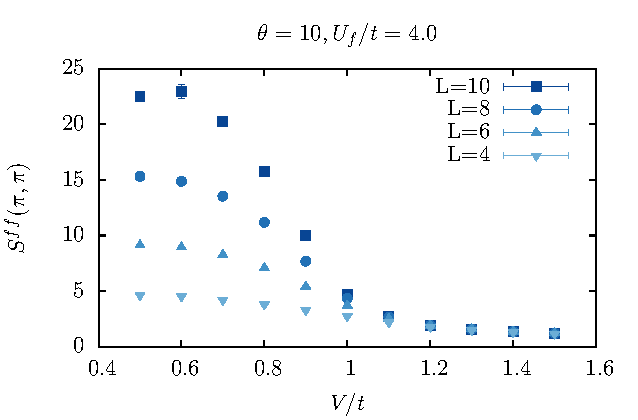
\includegraphics[width=0.6\textwidth]{Figures/PAM/PAM.pdf}

\caption{The periodic Anderson model.  Here we  plot the  equal-time spin structure factor  of the f-electrons  at $\ve{q} = (\pi,\pi)$.   This quantity is found in the file \texttt{SpinZ\_eqJK}.  The  pyALF  based python script    \href{https://git.physik.uni-wuerzburg.de/ALF/pyALF/-/blob/master/Scripts/Hubbard_PAM.py}{\texttt{Hubbard\_PAM.py}}  produces the data  shown for the $L=8$ lattice.    One sees  that for the chosen value of $U_f/t$  the competition between the RKKY interaction and  Kondo screening drives the system through a magnetic order-disorder transition at $V_c/t \simeq 1$  \cite{Vekic95}.}
        \label{Fig:PAM}
\end{figure}



%{\color{red}  If we do a good job in the previous sections we actually do not need much more explanation for this.   We could also provide Juypyter notebooks to start a set of Hubbard  hamiltonians.  e.g.  
%\begin{itemize}
%\item   \texttt{Pam\_square.ipynb}            SU(N) Square lattice PAM 
%\item  \texttt{Pam\_honeycomb.ipynb}     SU(N) Honeycomb lattice lattice PAM 
%\item  \texttt{Bilayer\_Hubbard.ipynb}      SU(N) Hubbard model on bilayers.
%\item  \texttt{N\_leg\_ladder\_Hubbard.ipynb}   SU(N) n-leg-ladder  Hubbard
%\item ...
%\end{itemize} 
%Would be nice to discuss this point.}


\subsection{O(2N)  t-V models  \texttt{tV\_mod.F90}}

%This would include the SU(N)  $t-V$ models on various lattices.  The defining property of this set of Hamiltonians would be the enlarged O(2N) symmetry.  Again  this   module should support our standard bipartite lattices. 

The parameter space for this model class  reads: 

\begin{lstlisting}[style=fortran,escapechar=\#,breaklines=true]
&VAR_tV                    !! Variables for the t-V class
ham_T     = 1.d0            ! Hopping parameter
ham_chem  = 0.d0            ! Chemical potential
ham_V     = 0.5d0           ! interaction strength
ham_T2    = 1.d0            ! For bilayer systems
ham_V2    = 0.5d0           ! For bilayer systems
ham_Tperp = 1.d0            ! For bilayer systems
ham_Vperp = 0.5d0           ! For bilayer systems
/

\end{lstlisting}
In the above   \texttt{ham\_T} and \texttt{ham\_T2} and \texttt{ham\_Tperp}   correspond to the hopping in the first and second layers respectively and  \texttt{ham\_Tperp}   is to the interlayer hopping.   The interaction term has an orbital index, 
\texttt{ham\_V}  for the first and  \texttt{ham\_V2}  for the second layers,  and \texttt{ham\_Vperp} for interlayer coupling. Note the we use the same sign conventions here for both the hopping parameters and the interaction strength. This implies a relative minus sign between here and the $U_\delta$ interaction strength of the Hubbard model (see Sec.~\ref{sec:hubbard}).
Finally   \texttt{ham\_chem}  corresponds to the chemical potential. Let us define the operator
\begin{equation}
\hat{b}_{\langle (\ve{i},\ve{\delta}), (\ve{j},\ve{\delta}') \rangle} =  \sum_{\sigma =1}^{N}    \hat{c}^{\dagger}_{(\ve{i},\ve{\delta}), \sigma }   e^{\frac{2 \pi i}{\Phi_0} \int_{\ve{i} + \ve{\delta}}^{\ve{j} + \ve{\delta}'}  
	\vec{A}(\ve{l})  d \ve{l}} \hat{c}^{}_{(\ve{j},\ve{\delta}'),\sigma} 
+ \textrm{H.c.}
\end{equation}
The model is then defined as follows:
\begin{align}
\hat{H}= & \sum_{\langle (\ve{i},\ve{\delta}), (\ve{j},\ve{\delta}') \rangle}   T_{(\ve{i},\ve{\delta}), (\ve{j},\ve{\delta}')}    \hat{b}_{\langle (\ve{i},\ve{\delta}), (\ve{j},\ve{\delta}') \rangle}
+ \sum_{\langle (\ve{i},\ve{\delta}), (\ve{j},\ve{\delta}') \rangle}  \frac{V_{(\ve{i},\ve{\delta}), (\ve{j},\ve{\delta}')}}{N} \left(  \hat{b}_{\langle (\ve{i},\ve{\delta}), (\ve{j},\ve{\delta}') \rangle}  \right)^2  \nonumber \\
& - \mu \sum_{(\ve{i},\ve{\delta})}  \sum_{\sigma =1}^{N} \hat{c}^{\dagger}_{(\vec{i},\ve{\delta}),\sigma } \hat{c}^{\phantom\dagger}_{(\vec{i},\ve{\delta}),\sigma } \,.
\end{align}
The generic hopping is taken from Eq.~\eqref{generic_hopping.eq} with appropriate boundary conditions given by Eq.~\eqref{generic_boundary.eq}. The index $\ve{i}$ runs over the unit cells, $\ve{\delta}$ over the orbitals in each unit cell and $\sigma$  from $1$ to $N$,  encoding the SU(N) symmetry.
Note that $N$ corresponds to \texttt{N\_SUN}  in the code.
The flavor index is set to unity such that it does not appear in the  Hamiltonian.
The chemical potential $\mu$ is relevant only for the finite temperature code.
An example showing how to run this model class can be found in the pyALF based Jupyter notebook   
\href{https://git.physik.uni-wuerzburg.de/ALF/pyALF/-/blob/master/Notebooks/tV_model.ipynb}{\texttt{tV\_model.ipynb}}.

As a concrete example, we can consider the Hamiltonian of the t-V model of SU(N) fermions on the square lattice,
\begin{align}
\hat{H}= & -t \sum_{\langle \ve{i}, \ve{j} \rangle}  \hat{b}_{\langle \ve{i}, \ve{j} \rangle}
- \frac{V}{N} \sum_{\langle \ve{i}, \ve{j} \rangle}  \left(  \hat{b}_{\langle \ve{i}, \ve{j} \rangle}  \right)^2   - \mu \sum_{\ve{i}}  \sum_{\sigma =1}^{N} \hat{c}^{\dagger}_{\vec{i},\sigma } \hat{c}^{\phantom\dagger}_{\vec{i},\sigma } \,,
\end{align} 
which can be simulated by setting $\texttt{ham\_T}=t$, $\texttt{ham\_V} = V$, and $\texttt{ham\_chem}=\mu$.
At half-band filling $\mu =0$, the sign problem is absent for $V>0$ and for all values of $N$.  For even values of $N$ no sign problem occurs for $V>0$ and arbitrary chemical potentials.   

Note  that  in the absence of orbital magnetic fields,  the model has an $O(2N)$ symmetry. This can be seen by writing the model in a Majorana basis (see e.g. Ref.~\cite{Assaad16}). 

%%%%%%%%%%%%%%%%%%%%%%%%%%%%%%%%%%%%%%%%%%%%%%%%%%%%%%%%%%%%%%%%%
% Copyright (c) 2016 2017 The ALF project.
% This is a part of the ALF project documentation.
% The ALF project documentation by the ALF contributors is licensed
% under a Creative Commons Attribution-ShareAlike 4.0 International License.
% For the licensing details of the documentation see license.CCBYSA.
% !TEX root = Model_classes.tex 


The Kondo lattice model we consider reads is an SU(N) generalization of the SU(2) Kondo-model   discussed in \cite{Capponi00,Assaad99a}.   Here we follow the work of  Ref.~\cite{Raczkowski20}. Let 
$T^{a}$ be the  $N^2 -1  $ generators of SU($N$)   that  satisfy the normalization condition: 
\begin{equation}
	\text{Tr}  \left[ T^{a} T^{b} \right]   = \frac{1}{2}\delta_{a,b}.
\label{Normalization_condition.eq}
\end{equation}
For the SU(2) case $T^{a}$  corresponds to the $T  = \frac{1}{2} \ve{\sigma}$ with $\ve{\sigma}$   a vector of the three Pauli spin matrices.      The   Hamiltonian is defined on bilayer  square or honeycomb lattices, with  hopping restricted to the  first layer  (i.e  conduction orbitals $\ve{c}^{\dagger}_{i}  )$   and  spins, f-orbitals, on the second layer. 
\begin{equation}
	\hat{H}     =   - t  \sum_{\langle i,j \rangle}    \sum_{\sigma=1}^{N}  \left(  \hat{c}^{\dagger}_{i,\sigma}  e^{\frac{2\pi i}{\Phi_0}  \int_{i}^{j} \ve{A}\cdot d \ve{l}}\hat{c}^{\phantom\dagger}_{j,\sigma}   + H.c.  \right)  - \mu \sum_{i,\sigma} \hat{c}^{\dagger}_{i,\sigma}  \hat{c}^{\phantom\dagger}_{i,\sigma} 
	+    \frac{U_c}{N}  \sum_{i}   \left( \hat{n}^c_i -  \frac{N}{2} \right)^2  
         +  \frac{2 J}{N} \sum_{i, a=1  }^{N^2 -1}  \hat{T}^{a,c}_{i}  \hat{T}^{a,f}_{i}. 
\label{Kondo_SUN_Ham.eq}
\end{equation}
In the above,  $i$ is a super-index  accounting for the unit cell and orbital,
\begin{equation}
	 \hat{T}^{a,c}_{i}   =   \sum_{\sigma,\sigma'=1}^{N} \hat{c}^{\dagger}_{i,\sigma}T^{a}_{\sigma,\sigma'}  \hat{\ve{c}}^{\phantom\dagger}_{i,\sigma'}, \; \; 
	  \hat{T}^{a,f}_{i}   = \sum_{\sigma,\sigma'=1}^{N} \hat{f}^{\dagger}_{i,\sigma} T^{a}_{\sigma,\sigma'}  \hat{f}^{\phantom\dagger}_{i,\sigma'},  
	  \text{   and  }   \hat{n}^c_i  = \sum_{\sigma=1}^{N} \hat{c}_{i,\sigma}^{\dagger} \hat{c}_{i,\sigma}^{\phantom\dagger} 
\end{equation}
Finally, the constraint, 
\begin{equation}
   \sum_{\sigma=1}^{N}  \hat{f}^{\dagger}_{i,\sigma}   \hat{f}^{\phantom\dagger}_{i,\sigma}     = \frac{N}{2}
\end{equation}
holds.

Some  rewriting has to be carried out so as to implement  the model.   First, we  use the  relation:
\begin{equation*}
	\sum_{a} T^{a}_{\alpha,\beta} T^{a}_{\alpha',\beta'} = \frac{1}{2} \left(  \delta_{\alpha,\beta'}  \delta_{\alpha',\beta} - \frac{1}{N} \delta_{\alpha,\beta} \delta_{\alpha', \beta'} \right), 
\end{equation*}
to  show that  in the unconstrained Hilbert space,
\begin{align}
	 \frac{2 J}{N} \sum_{ a=1  }^{N^2 -1}  \hat{T}^{a,c}_{i}  \hat{T}^{a,f}_{i}   = &   - \frac{J}{2N} \sum_{i}  \left( 
                \hat{D}^{\dagger}_{i} \hat{D}^{\phantom\dagger}_{i}   +    \hat{D}^{\phantom\dagger}_{i} \hat{D}^{\dagger}_{i}    \right)    + \frac{J}{N}   \left(   \frac{\hat{n}^{c}_i}{2}  + \frac{\hat{n}^{f}_i}{2} -  \frac{\hat{n}^{c}_i \hat{n}^{f}_i}{N}   \right) \nonumber 
 \end{align}
with
\begin{equation*}
	   \hat{D}^{\dagger}_{i}   =  \sum_{\sigma=1}^{N} \hat{c}^{\dagger}_{i,\sigma}  \hat{f}^{\phantom\dagger}_{i,\sigma}   \text{  and  }   \hat{n}^{f}_i =   \sum_{\sigma=1}^{N}    \hat{f}^{\dagger}_{i,\sigma}   \hat{f}^{\phantom\dagger}_{i,\sigma}.
\end{equation*}
In the constrained Hilbert space, $\hat{n}^{f}_i = N/2 $, the above gives:
\begin{align}
	 \frac{2 J}{N} \sum_{ a=1  }^{N^2 -1}  \hat{T}^{a,c}_{i}  \hat{T}^{a,f}_{i}   =     -  \frac{J}{4N}    \left[ \left(   \hat{D}^{\dagger}_{i}  + \hat{D}^{\phantom\dagger}_{i}    \right)^{2}  + 
                                                       \left(  i\hat{D}^{\dagger}_{i}  - i  \hat{D}^{\phantom\dagger}_{i}    \right)^2  \right] + \frac{J}{4}.  
 \end{align}
The  prefect square form  complies with the standards of the ALF.      We still have to impose the constraint. To do so, we   work in the unconstrained Hilbert  and add a Hubbard  U-term on  the f-orbitals.    With this addition, the Hamiltonian we simulate reads: 

\begin{align}
	\hat{H}_{QMC}      =  &   - t  \sum_{\langle i,j \rangle}    \sum_{\sigma=1}^{N}  \left(  \hat{c}^{\dagger}_{i,\sigma}  e^{\frac{2\pi i}{\Phi_0}  \int_{i}^{j} \ve{A}\cdot d \ve{l}}\hat{c}^{\phantom\dagger}_{j,\sigma}   + H.c.  \right)  - \mu \sum_{i,\sigma} \hat{c}^{\dagger}_{i,\sigma}  \hat{c}^{\phantom\dagger}_{i,\sigma} 
	+    \frac{U_c}{N}  \sum_{i}   \left( \hat{n}^c_i -  \frac{N}{2} \right)^2   \nonumber \\
          & -  \frac{J}{4N}    \left[ \left(   \hat{D}^{\dagger}_{i}  + \hat{D}^{\phantom\dagger}_{i}    \right)^{2}  + 
                                                       \left(  i\hat{D}^{\dagger}_{i}  - i  \hat{D}^{\phantom\dagger}_{i}    \right)^2  \right]  
       +    \frac{U_f}{N}  \sum_{i}   \left( \hat{n}^f_i -  \frac{N}{2} \right)^2.
\label{Kondo_SUN_Ham_QMC.eq}
\end{align}
The key point for the efficiency of the code, is to  see that 
\begin{equation}
	\left[   \hat{H}_{QMC},  \left( \hat{n}^f_i -  \frac{N}{2} \right)^2  \right]    = 0 
\label{Constraint_KLM.eq}
\end{equation}
such that the  constraint is implemented  efficiently.  In fact, for the finite temperature code  at inverse temperature $\beta$,  the unphysical Hilbert space   is suppressed by a  
factor  $e^{- \beta U_f/N} $. 





\subsubsection*{ The SU(2) case } 
The SU(2) case is special and allows for a more efficient implementation than  mentioned above.    The  key point is that  for the SU(2) case, the  Hubbard term is  related to  the fermion parity,
\begin{equation} 
   \left(   \hat{n}^f_i - 1 \right)^2    = \frac{  (-1)^{\hat{n}^f_i}  +1 }{2}
\end{equation}
such that we can omit the \textit{current}-term  $ \left(  i\hat{D}^{\dagger}_{i}  - i  \hat{D}^{\phantom\dagger}_{i}    \right)^2 $    without violating  Eq.~\ref{Constraint_KLM.eq}.  
As in Refs.~ \cite{Assaad99a,Capponi00,Beach04}.  
the Hamiltonian that one will simulate reads: 
 \begin{align}
 \label{eqn:ham_kondo}
 	\hat{\mathcal{H}}  = &
	\underbrace{-t \sum_{\langle i,j \rangle,\sigma} \left( \hat{c}_{i,\sigma}^{\dagger} e^{\frac{2\pi i}{\Phi_0}  \int_{i}^{j} \ve{A}\cdot d \ve{l}} \hat{c}_{j,\sigma}^{\phantom\dagger}   + \text{H.c.} \right) +
	  \frac{U_c}{2}   \sum_{i}   \left( \hat{n}^{c}_{i} -1 \right)^2    }_{\equiv \hat{\mathcal{H}}_{tU_c}}     \nonumber \\   & -  \frac{J}{4} 
	\sum_{i} \left( \sum_{\sigma} \hat{c}_{i,\sigma}^{\dagger}  \hat{f}_{i,\sigma}^{\phantom\dagger}  + 
	                                                        \hat{f}_{i,\sigma}^{\dagger}  \hat{c}_{i,\sigma}^{\phantom\dagger}   \right)^{2}   +
        \underbrace{\frac{U_f}{2}   \sum_{i}   \left( \hat{n}^{f}_{i} -1 \right)^2}_{\equiv \hat{\mathcal{H}}_{U_f}}.
 \end{align}
The  relation to the Kondo lattice model follows  from expanding the square  of the hybridization to obtain: 
 \begin{equation}
 	\hat{\mathcal{H}}  =\hat{\mathcal{H}}_{tU_c}   
	+ J \sum_{\vec{i}}  \left(  \hat{\vec{S}}^{c}_{\vec{i}} \cdot  \hat{\vec{S}}^{f}_{\vec{i}}    +   \hat{\eta}^{z,c}_{\vec{i}} \cdot  \hat{\eta}^{z,f}_{\vec{i}}  
		-  \hat{\eta}^{x,c}_{\vec{i}} \cdot  \hat{\eta}^{x,f}_{\vec{i}}  -  \hat{\eta}^{y,c}_{\vec{i}} \cdot  \hat{\eta}^{y,f}_{\vec{i}} \right) 
	 + \hat{\mathcal{H}}_{U_f}.
 \end{equation}
 where the $\eta$-operators  relate to the spin-operators via a particle-hole transformation in one spin sector: 
 \begin{equation} 
 	\hat{\eta}^{\alpha}_{\vec{i}}  = \hat{P}^{-1}  \hat{S}^{\alpha}_{\vec{i}} \hat{P}  	\; \text{ with }  \;   
	\hat{P}^{-1}  \hat{c}^{\phantom\dagger}_{\vec{i},\uparrow} \hat{P}  =   (-1)^{i_x+i_y} \hat{c}^{\dagger}_{\vec{i},\uparrow}  \; \text{ and }  \;   
	\hat{P}^{-1}  \hat{c}^{\phantom\dagger}_{\vec{i},\downarrow} \hat{P}  = \hat{c}^{\phantom\dagger}_{\vec{i},\downarrow} 
 \end{equation}
 Since the $\hat{\eta}^{f} $- and $ \hat{S}^{f} $-operators  do not alter the  parity [$(-1)^{\hat{n}^{f}_{\vec{i}}}$ ] of the $f$-sites, 
 \begin{equation}
 	\left[  \hat{\mathcal{H}}, \hat{\mathcal{H}}_{U_f} \right] = 0.
 \end{equation}
 Thereby,  and for positive values of $U$ ,  doubly occupied  or empty $f$-sites -- corresponding to even parity sites -- are suppressed  by a  Boltzmann factor 
 $e^{-\beta U_f/2} $ in comparison to odd parity sites.   Choosing $\beta U_f $ adequately essentially allows to  restrict the Hilbert space to  odd parity $f$-sites.  
 In this Hilbert space $\hat{\eta}^{x,f} = \hat{\eta}^{y,f} =  \hat{\eta}^{z,f} =0$  such that the Hamiltonian (\ref{eqn:ham_kondo}) reduces to the Kondo lattice model. 

%An implementation of the Kondo Lattice model on the  Honeycomb lattice with additional z-z frustration considered in Ref.~\cite{SatoT17_1}, 
%\begin{equation}
%\hat{H}_{\text{Spin}} = J^{z}\sum_{\langle \langle i,j \rangle \rangle}\hat{S}_{i}^{z}\hat{S}_{j}^{z},  \hfill  \hat{H}_{\text{Fermion}} = -t\sum_{\langle i,j \rangle,\sigma}\hat{c}_{i\sigma}^\dagger \hat{c}^{\phantom\dagger} _{j\sigma},  \hfill
%\hat{H}_{\text{Kondo}}  =  J^{\text{K}} \sum_{i}    \frac{1}{2} \hat{\pmb{c}}^{\dagger}_{i} \pmb{\sigma}\hat{\pmb{c}}^{\phantom\dagger}_{i} \cdot \hat{{\bm S}}^{\phantom\dagger} _{i} , \hfill
%\end{equation}
%can be found in  the \texttt{Hamiltonian\_Kondo\_Honey\_mod.F90}

\subsubsection*{ QMC implementation } 

The parameter space for this model class  reads: 

\begin{lstlisting}[style=fortran,escapechar=\#,breaklines=true]
&VAR_Kondo                 !! Variables for the Kondo  class
ham_T     = 1.d0            ! Hopping parameter
ham_chem  = 0.d0            ! Chemical potential
ham_U     = 0.d0            ! Hubbard interaction  on  c-orbitals Uc
ham_U2    = 2.d0            ! Hubbard interaction  on  f-orbials  Uf
ham_JK    = 2.d0            ! Kondo Coupling  J
/
\end{lstlisting}



%%%%%%%%%%%%%%%%%%%%%%%%%%%%%%%%%%%%%%%%%%%%%%%%%%%%%%%%%%%%%%%%%

%%%%%%%%%%%%%%%%%%%%%%%%%%%%%%%%%%%%%%%%%%%%%%%%%%%%%%%%%%%%%%%%%
% Copyright (c) 2016-2020 The ALF project.
% This is a part of the ALF project documentation.
% The ALF project documentation by the ALF contributors is licensed
% under a Creative Commons Attribution-ShareAlike 4.0 International License.
% For the licensing details of the documentation see license.CCBYSA.
% !TEX root = Model_classes.tex 

The model we consider  here is  defined  for \texttt{N\_FL=1},  arbitrary values of \texttt{N\_SUN}  and  supports all the predefined lattices.  It  reads: 
\begin{equation}
\hat{H}=  \sum_{i,j}  \sum_{\sigma =1}^{N}  T_{i, j}    \hat{c}^{\dagger}_{i, \sigma }   e^{\frac{2 \pi i}{\Phi_0} \int_{i}^{j}  
     \vec{A}(\ve{l})  d \ve{l}} \hat{c}^{}_{j,\sigma}   +
     \frac{1} { N } \sum_{i,j}  \left(  \hat{n}_{i} -  \frac{N}{2}  \right)  V_{i,j} \left(  \hat{n}_{j} -  \frac{N}{2}  \right)
      - \mu \sum_{i} \hat{n}_{i} 
\end{equation}
In the above,  $i = (\ve{i}, \ve{\delta}_i) $  and $j = (\ve{j}, \ve{\delta}_j) $  are super-indices encoding the unit-cell and orbital and 
$  \hat{n}_{i} = \sum_{\sigma =1}^{N} \hat{c}^{\dagger}_{i,\sigma } \hat{c}^{\phantom\dagger}_{i,\sigma} $ For simplicity, the interaction is specified by  two  parameters, $U$ and $\alpha$ that monitor the  strength of the onsite interaction and the magnitude of the Coulomb tail  respectively.  
\begin{equation}
	V_{i, j}     \equiv V(\vec{i}  + \vec{\delta}_i ,  \vec{j}  + \vec{\delta}_j  )  =   U \left\{
	\begin{array}{ll}  
	1          &   \text{ if }  i = j    \\
	\frac{\alpha   \;   d_\mathrm{min}}{  {  || \vec{i} - \vec{j} + \vec{\delta}_i - \vec{\delta}_j  ||}   } &     \text{ otherwise }
	\end{array}
\right.
\end{equation}
Here $d_\mathrm{min}$ is the minimal distance between two orbitals.      On a  torus, some care  has be taken in  defining the distance. Let the lattice size be given by the vectors $\ve{L}_1$  and  $\ve{L}_2$  (see Sec.~\ref{sec:predefined_lattices}).  Then 
\begin{equation}
	|| \ve{i} || = \min_{n_1,n_2 \in \mathbb{Z} }  | \ve{i} - n_1 \ve{L}_1 -  n_2 \ve{L}_2 | 
\end{equation}
The implementation follows Ref.~\cite{Hohenadler14}  but now supports various lattice geometries.  We use  the following  HS decomposition:
\begin{equation}
e^{-\Delta \tau \hat{H}_V }  \propto \int \prod_{i} d \phi_{i}   e^{ - \frac{N \Delta \tau} {4} \sum_{i,j} \phi_{i} V^{-1}_{i,j}  \phi_{j} - \sum_{i}  i \Delta \tau \phi_i \left( \hat{n}_{i} - \frac{N}{2} \right) } 
\end{equation}
where $\phi_i $ is a  real  variable, $V$ is symmetric, and importantly has to be  positive definite  for the Gaussian integration to be defined. 
The partition function  reads:
\begin{equation}
	Z \propto \int \prod_{i} d \phi_{i, \tau} \overbrace{e^{ - \frac{N \Delta \tau} {4} \sum_{i,j} \phi_{i,\tau} V^{-1}_{i,j}  \phi_{j,\tau}} }^{W_B(\phi)}\underbrace{\text{Tr} \left[   \prod_{\tau}   
	 e^{-\Delta \tau \hat{H}_T}  e^{- \sum_{i}  i \Delta \tau \phi_{i,\tau} \left( \hat{n}_{i} - \frac{N}{2} \right) }\right]}_{W_F(\phi)}.
\end{equation}
such that the weight splits into a bosonic and fermionic parts. 
 
%In the above, the field has acquired time index. 
%{\color{red}   There is a constant to be fixed in the above equation}
 
For the update, it is convenient to  work in a basis where  $V$   is diagonal: 
\begin{equation}
	\text{ Diag}  \left( \lambda_1, \cdots ,\lambda_{\texttt{Ndim}} \right)    =  O^{T} V O 
\end{equation}
 with $O^T O = 1$  and define:
 \begin{equation}
 	  \eta_{i,\tau}^{\phantom\dagger}   =  \sum_{j} O^{T}_{i,j} \phi_{j,\tau}^{\phantom\dagger}.
 \end{equation}
 On a given time slice, $\tau_u$, we propose a  new field configuration with the probability: 
 \begin{equation}
 	T^{0} ( \eta  \rightarrow  \eta' ) = 
	\left\{ 
	\begin{array}{ll} 
	  \prod_{i} \left[  P P_B(\eta'_{i,\tau_u})  + (1-P) \delta( \eta_{i,\tau_u} - \eta'_{i,\tau_u})   \right]  & \text{  for  } \tau = \tau_u \\
	  \delta( \eta_{i,\tau} - \eta'_{i,\tau})   & \text{  for  } \tau \neq \tau_u 
	  \end{array}
	  \right.
 \end{equation}
 where 
 \begin{equation}
 	 P_B(\eta_{i,\tau})   \propto e^{ - \frac{N \Delta \tau} {4 \lambda_i}  \eta_{i,\tau}^2 },
 \end{equation}
$ P \in \left[0,1 \right] $ and $\delta $  corresponds to  the Dirac $\delta$-function.    That is, we  carry out  simple sampling of the field with probability $P$  and leave the field unchanged with probability 
$(1-P)$.  $P$ is a free parameter that   does not change the final result but that allows to adjust the acceptance.    We then use  the Metropolis-Hasting    acceptance-rejection  scheme   and accept the move  with probability 
\begin{equation}
   \text{min} \left(     \frac{T^{0} ( \eta'  \rightarrow \eta ) W_B(\eta') W_F(\eta')  }{ T^{0} ( \eta \rightarrow \eta' ) W_B(\eta) W_F(\eta) } , 1 \right)     = \text{min} \left(     \frac{W_F(\eta')  }{ W_F(\eta) } , 1 \right) . 
\end{equation}
where 
\begin{equation}
  W_B(\eta)  = e^{ - \frac{N \Delta \tau} {4 } \sum_{i,\tau} \eta_{i,\tau}^2/\lambda_i } 
  \text{   and   } 
  W_F(\eta)  = \text{Tr} \left[   \prod_{\tau}   
     e^{-\Delta \tau \hat{H}_T}  e^{- \sum_{i,j}  i \Delta \tau O_{i,j}\eta_{j,\tau} \left( \hat{n}_{i} - \frac{N}{2} \right) }\right]
\end{equation}


Since a local change on  a single time slice in the $\eta$ basis corresponds to a non-local in space update  in the $\phi$ basis, we  use the global update in  space routine to carry out the update (see Sec.~\ref{sec:global_space}). 

\subsubsection*{ QMC implementation } 

The name space for this model class  reads: 

\begin{lstlisting}[style=fortran,escapechar=\#,breaklines=true]
&VAR_LRC                   !! Variables for the  Long Range Coulomb class
ham_T          = 1.0       ! Specifies the hopping and chemical potential
ham_T2         = 1.0       ! For bilayer systems
ham_Tperp      = 1.0       ! For bilayer systems
ham_chem       = 1.0       ! Chemical potential
ham_U          = 4.0       ! On-site interaction
ham_alpha      = 0.1       ! Coulomb tail magnitude
Percent_change = 0.1       ! Parameter P 
/
\end{lstlisting}

By setting $\alpha$ to zero we can test this code against the Hubbard code.   For a   $ 4 \times 4 $ square  lattice at $ \beta t = 5$, $U/t = 4$, and half-band filling,     \texttt{Hamiltonian\_Hubbard\_mod.F90}    gives $ E = -13.188896      \pm  0.001698 $  and
  \texttt{Hamiltonian\_LRC\_mod.F90}  $ E =  -13.198512    \pm  0.040029 $.    Note that for the  Hubbard code we have used  the default \texttt{Mz = True}.   This  option   breaks SU(2) spin symmetry for a given HS configuration but produces very precise values of the energy. On the other hand,  the LRC code  is an SU(2) invariant code ( as would be  choosing \texttt{Mz = False}  )  and  produces  more  fluctuations in the double occupancy.   This  partly explains the difference in  error  bars between the two codes. 
  
% The definition of  the Coulomb repulsion is as follows. 
%A general lattice site  \texttt{I,n}   where \texttt{I: 1...Latt\%N} is the unit cell and \texttt{ n = 1 ...Latt\_unit\%NORB}  the orbital  is given by: 
%\begin{lstlisting}[style=fortran]
%X_p(:) = Latt%list(I,1)*latt%a1_p(:)  + Latt%list(I,2)*latt%a2_p(:) 
%          +   Latt_unit%Orb_pos_p(no_j,:)
%\end{lstlisting}
%or in more compact notation $ \vec{i}  + \vec{\delta}_i $.   By definition \texttt{Latt\_unit\%Orb\_pos\_p(1,:)=0}.
%The Coulomb repulsion between points   $ \vec{i}  + \vec{\delta}_i $   and $ \vec{j}  + \vec{\delta}_j $   reads: 
%\begin{equation}
%	V(\vec{i}  + \vec{\delta}_i ,  \vec{j}  + \vec{\delta}_j  )  =  \frac{U d_\mathrm{min} \alpha}{  |  \overline{\vec{i} - \vec{j}} + \vec{\delta}_i - \vec{\delta}_j  |}  
%\end{equation}




%%%%%%%%%%%%%%%%%%%%%%%%%%%%%%%%%%%%%%%%%%%%%%%%%%%%%%%%%%%%%%%%%

%%%%%%%%%%%%%%%%%%%%%%%%%%%%%%%%%%%%%%%%%%%%%%%%%%%%%%%%%%%%%%%%%
% Copyright (c) 2016 2017 The ALF project.
% This is a part of the ALF project documentation.
% The ALF project documentation by the ALF contributors is licensed
% under a Creative Commons Attribution-ShareAlike 4.0 International License.
% For the licensing details of the documentation see license.CCBYSA.
% !TEX root = doc.tex 


\subsection{$\Ztwo$ lattice gauge theories coupled to fermion and $\Ztwo$ matter  \texttt{Z2\_mod.F90}} \label{Z2.Sec}

The Hamiltonian we will consider here reads
\begin{align}
	\hat{H} =& -  t_{\Ztwo} \sum_{\langle \vec{i}, \vec{j} \rangle, \sigma } \hat{\sigma}^z_{\langle \vec{i}, \vec{j} \rangle}
	\left(\hat{\Psi}^{\dagger}_{\vec{i},\sigma} \hat{\Psi}^{\phantom{\dagger}}_{\vec{j},\sigma}   + h.c. \right) - \mu \sum_{\vec{i},\sigma} \hat{\Psi}^{\dagger}_{\vec{i},\sigma} \hat{\Psi}^{\phantom{\dagger}}_{\vec{i},\sigma}  
	-g \sum_{\langle \vec{i}, \vec{j} \rangle } \hat{\sigma}^{x}_{\langle \vec{i}, \vec{j} \rangle } \nonumber \\
	  & +K \sum_{\square} \prod_{\langle \vec{i}, \vec{j} \rangle \in \partial \square} \hat{\sigma}^{z}_{\langle \vec{i}, \vec{j} \rangle}  
	 + J  \sum_{\langle \vec{i}, \vec{j} \rangle}  \hat{\tau}^z_{\pmb{i}}  \hat{\sigma}^{z}_{\langle \vec{i}, \vec{j} \rangle} \hat{\tau}^z_{\pmb{j}}   
	      -  h \sum_{ \vec{i} } \hat{\tau}^x_{\vec{i}} \nonumber \\
	& - t  \sum_{\langle \vec{i}, \vec{j} \rangle, \sigma }   \hat{\tau}^z_{\pmb{i}}   \hat{\tau}^z_{\pmb{j}}  \left( \hat{\Psi}^{\dagger}_{\vec{i},\sigma} \hat{\Psi}^{\phantom{\dagger}}_{\vec{j},\sigma} 	+ h.c. \right) + \frac{U}{N}\sum_{\ve{i}} \left[ \sum_{\sigma}  \left( \hat{\Psi}^{\dagger}_{\ve{i},\sigma}  \hat{\Psi}^{\phantom\dagger}_{\ve{i},\sigma} - 1/2\right) \right]^2.
\end{align}  
The model is defined on a square lattice, and describers fermions, 
\begin{align}
 \left\{ \hat{\Psi}^{\dagger}_{\vec{i},\sigma},  \hat{\Psi}^{\phantom\dagger}_{\vec{j},\sigma'} \right\}  = \delta_{\vec{i},\vec{j}} \delta_{\sigma,\sigma'}, \;  
\left\{ \hat{\Psi}^{\phantom\dagger}_{\vec{i},\sigma},  \hat{\Psi}^{\phantom\dagger}_{\vec{j},\sigma'} \right\}  =  0,  
\end{align}
coupled to  bond gauge fields, 
\begin{align}
\hat{\sigma}^{z}_{\langle \vec{i}, \vec{j} \rangle}  = 
\begin{bmatrix}
1 & 0 \\
0 & -1 
\end{bmatrix},  
\hat{\sigma}^x_{\langle \vec{i}, \vec{j} \rangle}  = 
\begin{bmatrix}
0 & 1 \\
1 & 0 
\end{bmatrix},   
\left\{ \hat{\sigma}^{z}_{\langle \vec{i}, \vec{j} \rangle} , \hat{\sigma}^x_{\langle \vec{i}', \vec{j}'  \rangle} \right\}  =  2 \left( 1 -  \delta_{\langle \vec{i}, \vec{j}  \rangle, \langle \vec{i}', \vec{j}'  \rangle } \right) 
\hat{\sigma}^{z}_{\langle \vec{i}, \vec{j} \rangle}  \hat{\sigma}^x_{\langle \vec{i}', \vec{j}'  \rangle}
\end{align}
and  $\Ztwo$ matter fields:
\begin{align}
 \hat{\tau}_{\ve{i}}^{z} = 
\begin{bmatrix}
1 & 0 \\
0 & -1 
\end{bmatrix},\quad
\hat{\tau}^{x}_{\vec{i} }  = 
\begin{bmatrix}
0 & 1 \\
1 & 0 
\end{bmatrix},\quad 
\left\{ \hat{\tau}^{z}_{ \vec{i} }, \hat{\tau}^x_{\vec{i}'} \right\}  =  2 \left( 1 -  \delta_{ \vec{i}, \vec{i}' } \right) 
\hat{\tau}^{z}_{ \vec{i} }  \hat{\tau}^x_{ \vec{i}' }.
\end{align}
 Fermions,  gauge fields and $\Ztwo$ matter fields commute with each other. 
 
 Importantly,  the model has a local  $\Ztwo$ symmetry. Consider:
\begin{equation}
	\hat{Q}_{\vec{i}} =  (-1)^{\sum_{\sigma} \hat{\Psi}^{\dagger}_{\vec{i},\sigma} \hat{\Psi}^{\phantom{\dagger}}_{\vec{i},\sigma}   } 
	\;  \hat{\tau}^{x}_{\vec{i}}  \; \hat{\sigma}^{x}_{\vec{i},\vec{i} +  \vec{a}_x} \hat{\sigma}^{x}_{\vec{i},\vec{i} -  \vec{a}_x} \hat{\sigma}^{x}_{\vec{i},\vec{i} +  \vec{a}_y} \hat{\sigma}^{x}_{\vec{i}}.
\end{equation} 
One can  then show that  $\hat{Q}_{\vec{i}}^2 = 1 $ and that
\begin{equation}
	\left[   \hat{Q}_{\vec{i}}, \hat{H}  \right]  = 0. 
\end{equation} 
The above allows us to assign $\Ztwo$  charges to the operators.   Since $ \left\{ \hat{Q}_{\vec{i}},   \hat{\Psi}^{\dagger}_{\vec{i},\sigma} \right\} =    0 $ we can assign a $\Ztwo$  charge to the fermions.  Equivalently 
$\hat{\tau}^{z}_{\ve{i}}$   has a $\Ztwo$ charge and $\hat{\sigma}^{z}_{\vec{i},\vec{j}} $   carries  $\Ztwo$ charges at its ends.   
 Since the total fermion number is conserved,   we can assign an electric charge to the  fermions.
Finally, the model has an SU(N) color symmetry.
In fact, at zero chemical potential and $U=0$, the symmetry is enhanced to $O(2N)$ \cite{Assaad16}.
Aspects of this Hamiltonian were investigated in Refs.~\cite{Assaad16,Gazit16,Gazit18,Gazit19,Hohenadler18,Hohenadler19} and we refer the interested user to these papers for a discussion of the phases and phase transitions supported by the model.

\subsubsection*{QMC implementation} 

The name space for this model class reads: 

\begin{lstlisting}[style=fortran,escapechar=\#,breaklines=true]
&VAR_Z2_Matter             !! Variables for the Z_2 class
ham_T          = 1.0        ! Hopping for fermions
ham_TZ2        = 1.0        ! Hopping for orthogonal fermions
ham_chem       = 0.0        ! Chemical potential for fermions
ham_U          = 0.0        ! Hubbard for fermions
Ham_J          = 1.0        ! Hopping Z2 matter fields
Ham_K          = 1.0        ! Plaquette term for gauge fields
Ham_h          = 1.0        ! sigma^x-term for matter
Ham_g          = 1.0        ! tau^x-term for gauge
Dtau           = 0.1d0      ! Thereby Ltrot=Beta/dtau
Beta           = 10.d0      ! Inverse temperature
Projector      = .False.    ! To enable projective code
Theta          = 10.0       ! Projection parameter 
/
\end{lstlisting}


We note that the implementation is such that  if \texttt{Ham\_T=0}   (\texttt{Ham\_TZ2=0}) then all the terms involving the matter field ($\Ztwo$  gauge field) are automatically set to zero.  
We warn the user that autocorrelation and warmup times can be  large for this model class.
At this point, only the finite temperature code is implemented. 

The key point to implement the model is to  define a new bond variable: 
\begin{equation}
	\hat{\mu}^{z}_{ \langle  \ve{i}, \ve{j}  \rangle }  =  \hat{\tau}^{z}_{ \ve{i}}\hat{\tau}^{z}_{\ve{j}  }. 
\end{equation}  
By construction, the $\hat{\mu}^{z}_{ \langle  \ve{i}, \ve{j}  \rangle } $ bond variables   have a zero flux constraint:
\begin{equation}
	\hat{\mu}^{z}_{ \langle  \ve{i}, \ve{i} + \ve{a}_x  \rangle }  \hat{ \mu}^{z}_{ \langle  \ve{i} + \ve{a}_x, \ve{i} + \ve{a}_x  + \ve{a}_y \rangle } 
	\hat{\mu}^{z}_{ \langle  \ve{i} + \ve{a}_x + \ve{a}_y, \ve{i} +  \ve{a}_y \rangle } \hat{\mu}^{z}_{ \langle  \ve{i} + \ve{a}_y, \ve{i}  \rangle }  = 1. 
\label{zero_flux.eq}
\end{equation} 


Consider a basis where  $\hat{\mu}^{z}_{ \langle  \ve{i}, \ve{j}  \rangle } $ and $  \hat{\tau}^{z}_{ \ve{i}}$  are diagonal with eigenvalues  $\mu_{ \langle  \ve{i}, \ve{j}  \rangle } $ and $  {\tau}_{ \ve{i}}$  respectively. 
The map from  $ \left\{ \tau_{\vec{i}}  \right\} $ to $ \left\{ \mu_{\langle \vec{i}, \vec{j} \rangle } \right\} $  is unique.
The reverse however  is valid only up to a global sign.
To pin down this sign (and thereby  the  relative signs between different time slices)  we store the fields $ \mu_{\langle \vec{i},\vec{j} \rangle } $ at every time slice as well as the value of the Ising field at a reference site $\tau_{\vec{i} = \ve{0}}$. Within the ALF, this can be done by adding a dummy operator in the \texttt{Op\_V} list to carry this degree of freedom.    With this extra degree of freedom we can switch  between the two representations without loosing any information.   To compute the Ising part of the action it is certainly more transparent to work  with the $ \left\{ \tau_{\vec{i}}  \right\} $  variables. For the  fermion determinant,  the $ \left\{ \mu_{\langle \vec{i}, \vec{j} \rangle } \right\} $   are more convenient.

Since flipping  $\hat{\tau}^{z}_{ \ve{i}} $  amounts to changing the sign of the four  bond variables emanating from site $\ve{i}$, the identity:
\begin{equation}
\hat{\tau}^x_{\ve{i}}  = \hat{\mu}^{x}_{\ve{i},\ve{i} + \ve{a}_x } \hat{\mu}^{x}_{\ve{i} + \ve{a}_x, \ve{i} + \ve{a}_x + \ve{a}_y }   \hat{\mu}^{x}_{\ve{i} + \ve{a}_x + \ve{a}_y, \ve{i} + \ve{a}_y  }
\end{equation}
holds.  
Note that $\left\{ \hat{\mu}^{z}_{\langle \vec{i}, \vec{j} \rangle} , \hat{\mu}^x_{\langle \vec{i}', \vec{j}'  \rangle} \right\}  =  2 \left( 1 -  \delta_{\langle \vec{i}, \vec{j}  \rangle, \langle \vec{i}', \vec{j}'  \rangle } \right) 
\hat{\mu}^{z}_{\langle \vec{i}, \vec{j} \rangle}  \hat{\mu}^x_{\langle \vec{i}', \vec{j}'  \rangle} $, such that applying $\hat{\mu}^x_{\langle \vec{i}, \vec{j}  \rangle}$  on an eigenstate of  $\hat{\mu}^{z}_{\langle \vec{i}, \vec{j} \rangle}$  flips the field. 


The model  can then be written as:
\begin{align}
	\hat{H} =& - t_{\Ztwo}\! \sum_{\langle \vec{i}, \vec{j} \rangle, \sigma } \hat{\sigma}^z_{\langle \vec{i}, \vec{j} \rangle}
	\left(\hat{\Psi}^{\dagger}_{\vec{i},\sigma} \hat{\Psi}^{\phantom{\dagger}}_{\vec{j},\sigma} \!+ h.c. \right) - \mu \sum_{\vec{i},\sigma} \hat{\Psi}^{\dagger}_{\vec{i},\sigma} \hat{\Psi}^{\phantom{\dagger}}_{\vec{i},\sigma}  
	-g \sum_{\langle \vec{i}, \vec{j} \rangle } \hat{\sigma}^{x}_{\langle \vec{i}, \vec{j} \rangle }  +
	  K \sum_{\square} \prod_{\langle \vec{i}, \vec{j} \rangle \in \partial \square} \hat{\sigma}^{z}_{\langle \vec{i}, \vec{j} \rangle}  \nonumber \\
	& + J  \sum_{\langle \vec{i}, \vec{j} \rangle}  \hat{\mu}^z_{ \langle \pmb{i}, \ve{j} \rangle }  \hat{\sigma}^{z}_{\langle \vec{i}, \vec{j} \rangle}    
	      -  h \sum_{ \vec{i} } \hat{\mu}^{x}_{\ve{i},\ve{i} + \ve{a}_x } \hat{\mu}^{x}_{\ve{i} + \ve{a}_x, \ve{i} + \ve{a}_x + \ve{a}_y }   \hat{\mu}^{x}_{\ve{i} + \ve{a}_x + \ve{a}_y, \ve{i} + \ve{a}_y  }
	         \hat{\mu}^{x}_{\ve{i} + \ve{a}_y, \ve{i}  }	\nonumber  \\      
	&        - t  \sum_{\langle \vec{i}, \vec{j} \rangle, \sigma }   \hat{\mu}^z_{\pmb{i},\ve{j}}    \left( \hat{\Psi}^{\dagger}_{\vec{i},\sigma} \hat{\Psi}^{\phantom{\dagger}}_{\vec{j},\sigma} 	+ h.c. \right) + \frac{U}{N}\sum_{\ve{i}} \left[ \sum_{\sigma}  ( \hat{\Psi}^{\dagger}_{\ve{i},\sigma}  \hat{\Psi}^{\phantom\dagger}_{\ve{i},\sigma} - 1/2 ) \right]^2 
\end{align}  
subject to the constraint of Eq.~\eqref{zero_flux.eq}.  

To formulate the Monte Carlo, we work in a basis in which  $\hat{\mu}^{z}_{ \langle  \ve{i}, \ve{j} \rangle }$,  $ \hat{\tau}^{z}_{   \ve{0} } $  and  $ \hat{\sigma}^{z}_{ \langle  \ve{i}, \ve{j} \rangle }$    are diagonal: 
\begin{align}
	  \hat{\mu}^{z}_{ \langle  \ve{i}, \ve{j} \rangle } |  \underline{s} \rangle  =  \mu_{ \langle  \ve{i}, \ve{j} \rangle }   |  \underline{s} \rangle,\quad 
	 \hat{\sigma}^{z}_{ \langle  \ve{i}, \ve{j} \rangle }|  \underline{s} \rangle  =  \sigma_{ \langle  \ve{i}, \ve{j} \rangle } |  \underline{s} \rangle,\quad    
	  \hat{\tau}^{z}_{   \ve{0} }  |  \underline{s} \rangle   =  \tau_{  \ve{0} } |  \underline{s} \rangle
\end{align}
with $ \underline{s} = \left( \left\{  \mu_{ \langle  \ve{i}, \ve{j} \rangle }  \right\},  \left\{  \sigma_{ \langle  \ve{i}, \ve{j} \rangle }  \right\},  \tau_{\ve{0}}  \right) $. 
In this basis,
\begin{equation}
   Z  =  \sum_{\underline {s}_1, \cdots, \underline {s}_{L_{\tau}}}  e^{-S_0( \left\{ \underline{s}_\tau \right\})} \text{Tr}_F   \left[    \prod_{\tau=1}^{L_{\tau}} e^{- \Delta \tau \hat{H}_F(\underline{s}_{\tau}) } \right],
 \end{equation}
 where 
 \begin{align*}
 	 S_0( \left\{ \underline{s}_\tau \right\})  = - \ln  \left[  \prod_{\tau=1}^{L_{\tau}}    \langle \underline{s}_{\tau+1}   |  e^{-\Delta \tau   \hat{H}_I} |  \underline{s}_{\tau}  \rangle  \right], 
\end{align*}
\begin{align*}
         \hat{H}_I  = &  -g \sum_{\langle \vec{i}, \vec{j} \rangle } \hat{\sigma}^{x}_{\langle \vec{i}, \vec{j} \rangle }  +
	                        K \sum_{\square} \prod_{\langle \vec{i}, \vec{j} \rangle \in \partial \square} \hat{\sigma}^{z}_{\langle \vec{i}, \vec{j} \rangle}  
	     + J  \sum_{\langle \vec{i}, \vec{j} \rangle}  \hat{\mu}^z_{ \langle \pmb{i}, \ve{j} \rangle }  \hat{\sigma}^{z}_{\langle \vec{i}, \vec{j} \rangle}     \\
	     & -  h \sum_{ \vec{i} } \hat{\mu}^{x}_{\ve{i},\ve{i} + \ve{a}_x } \hat{\mu}^{x}_{\ve{i} + \ve{a}_x, \ve{i} + \ve{a}_x + \ve{a}_y }   \hat{\mu}^{x}_{\ve{i} + \ve{a}_x + \ve{a}_y, \ve{i} + \ve{a}_y}  	
\end{align*}
and 
 \begin{align*}
   \hat{H}_F(\underline{s})  = 
   	     & - t_{\Ztwo} \sum_{\langle \vec{i}, \vec{j} \rangle, \sigma } \sigma_{\langle \vec{i}, \vec{j} \rangle}
	\left(\hat{\Psi}^{\dagger}_{\vec{i},\sigma} \hat{\Psi}^{\phantom{\dagger}}_{\vec{j},\sigma}   + h.c. \right) - \mu \sum_{\vec{i},\sigma} \hat{\Psi}^{\dagger}_{\vec{i},\sigma} \hat{\Psi}^{\phantom{\dagger}}_{\vec{i},\sigma}  \\
         & - t  \sum_{\langle \vec{i}, \vec{j} \rangle, \sigma }   \mu_{\pmb{i},\ve{j}}    \left( \hat{\Psi}^{\dagger}_{\vec{i},\sigma} \hat{\Psi}^{\phantom{\dagger}}_{\vec{j},\sigma} 	+ h.c. \right)  
         +\frac{U}{N}\sum_{\ve{i}} \left[ \sum_{\sigma}  ( \hat{\Psi}^{\dagger}_{\ve{i},\sigma}  \hat{\Psi}^{\phantom\dagger}_{\ve{i},\sigma} - 1/2 ) \right]^2. 
 \end{align*}
In the above, $  | \underline{s}_{L_\tau+1}  \rangle  = | \underline{s}_{1}  \rangle   $.  With a further  HS transformation of the Hubbard term (see Sec.~\ref{Hubbard_SUN_HS.eq})  the model is readily implemented in the ALF.    Including this HS field, $l$,  [see Eq.~\eqref{HS_squares}] yields  the configuration space: 
\begin{equation}
	C = \left(  \big\{  \mu_{ \langle  \ve{i}, \ve{j} \rangle,\tau }  \big\},  \big\{  \sigma_{ \langle  \ve{i}, \ve{j} \rangle, \tau }  \big\},    \big\{ \tau_{\ve{0},\tau}  \big\},  \big\{ l_{\ve{i}, \tau}  \big\}  \right) 
\end{equation} 
where the variables $\mu$, $\tau$ and $\sigma$ take the values $\pm 1$  and $l$  the values $\pm1, \pm 2$. 

The initial configuration as well as the  moves have to respect the zero flux constraint of Eq.~\eqref{zero_flux.eq}. Therefore, single spin flips of the $\mu$ fields  are prohibited and the minimal move one can carry out on  a given time slice is the following. We randomly choose a site $\vec{i} $ and  propose a move where:
$ \mu_{\vec{i},\vec{i} +  \vec{a}_x} \rightarrow - \mu_{\vec{i},\vec{i} +  \vec{a}_x} $,  $ \mu_{\vec{i},\vec{i} -  \vec{a}_x} \rightarrow - \mu_{\vec{i},\vec{i} -  \vec{a}_x} $,
$ \mu_{\vec{i},\vec{i} +  \vec{a}_y} \rightarrow - \mu_{\vec{i},\vec{i} +  \vec{a}_y} $ and $ \mu_{\vec{i},\vec{i} -  \vec{a}_y} \rightarrow - \mu_{\vec{i},\vec{i} -  \vec{a}_y} $.  One can carry out such moves by using the global move in real space option presented in Sec.~\ref{sec:global_space} and \ref{sec:input}.

\subsubsection{Projective approach} 
The program also supports a zero temperature implementation.
Our  choice  of the trial wave  function does not break any symmetries of the model and reads: 
\begin{equation}
	| \Psi_T \rangle  =    | \Psi^{F}_T \rangle \,  \otimes_{\langle \ve{i},\ve{j} \rangle}  | + \rangle_{\langle \ve{i},\ve{j} \rangle }     \,  \otimes_{ \ve{i} }  | + \rangle_{ \ve{i} }.   
\end{equation}
For the fermion part we use a Fermi sea with small dimerization to avoid the negative sign problem at half-filling (see Sec.~\ref{Sec:Plain_vanilla_trial}).  For the Ising part the trial   wave function  is diagonal in the $ \hat{\sigma}^{x}_{\langle \ve{i}, \ve{j} \rangle} $ and $\hat{\tau}^{x}_{\ve{i}} $   operators: 
\begin{equation}
	\hat{\sigma}^{x}_{\langle \ve{i}, \ve{j} \rangle}  | + \rangle_{\langle \ve{i},\ve{j} \rangle}  = | + \rangle_{\langle \ve{i},\ve{j} \rangle }  \quad\text{and}\quad  \hat{\tau}^{x}_{\ve{i}} | + \rangle_{ \ve{i} } = | + \rangle_{ \ve{i} }.
\end{equation}

An alternative  choice would  be to choose a  charge density wave  fermionic trial wave function.     This   violates the partial particle-hole symmetry of the model at $U=\mu=0$ and effectively imposes the constraint $\hat{Q}_{\ve{i}} =1 $.

\subsubsection{Observables} 
Apart from the  standard  observables discussed in Sec.~\ref{sec:predefined_observales}  the code computes additionally  
\begin{equation*} 
	\big\langle  \hat{\sigma}^{x}_{ \langle \ve{i},\ve{j} \rangle } \big\rangle    \quad\text{and}\quad  \big\langle  \hat{\tau}^{x}_{ \ve{j}  } \big\rangle,
\end{equation*}
which are written to file  \texttt{X\_scal}; 
\begin{equation*}
	\big\langle  \hat{\sigma}^{z}_{ \langle \ve{i},\ve{i} + \ve{a}_x \rangle }   \hat{\sigma}^{z}_{ \langle \ve{i} + \ve{a}_x ,\ve{i} + \ve{a}_x +  \ve{a}_y   \rangle }  
	\hat{\sigma}^{z}_{ \langle \ve{i}+ \ve{a}_x +  \ve{a}_y ,\ve{i} + \ve{a}_y \rangle }   \hat{\sigma}^{z}_{ \langle \ve{i} + \ve{a}_y,\ve{i}  \rangle }   \big\rangle
\end{equation*}
	and
\begin{equation*}
	\big\langle  \hat{\mu}^{z}_{ \langle \ve{i},\ve{i} + \ve{a}_x \rangle }   \hat{\mu}^{z}_{ \langle \ve{i} + \ve{a}_x ,\ve{i} + \ve{a}_x +  \ve{a}_y   \rangle }  
	\hat{\mu}^{z}_{ \langle \ve{i}+ \ve{a}_x +  \ve{a}_y ,\ve{i} + \ve{a}_y \rangle }   \hat{\mu}^{z}_{ \langle  \ve{i} + \ve{a}_y,\ve{i}  \rangle }   \big\rangle,
\end{equation*}
written to file \texttt{Flux\_scal}; and also $ \langle \hat{Q}_{\ve{i}} \rangle $ (file \texttt{Q\_scal}).  Note that the flux over a plaquette  of the $\hat{\mu}^{z}_{ \langle \ve{i},\ve{j} \rangle  } $   is equal to unity by construction  so that this observable  provides a sanity check.    The file \texttt{Q\_eq} contains the two-point correlation $ \langle \hat{Q}_{\ve{i}} \hat{Q}_{\ve{j}} \rangle -  \langle \hat{Q}_{\ve{i}} \rangle \langle \hat{Q}_{\ve{j}} \rangle $  and \texttt{Greenf\_eq}  the equal-time fermion   Green function 
$ \langle  \hat{\tau}^{z}_{\ve{i}}  \hat{\Psi}^{\dagger}_{\ve{i},\sigma}  \hat{\tau}^{z}_{\ve{j}}  \hat{\Psi}^{\phantom\dagger}_{\ve{j},\sigma}   \rangle $.


\subsubsection{A test case: $\Ztwo$ slave spin formulation of the SU(2) Hubbard model }

In this subsection, we  demonstrate that the code can be used to  simulate the attractive Hubbard model in the  $\Ztwo$-slave spin formulation \cite{Ruegg10}:
\begin{equation}
        \hat{H} = -t \sum_{\langle \vec{i}, \vec{j} \rangle, \sigma }\hat{c}^{\dagger}_{\vec{i},\sigma} \hat{c}^{\phantom{\dagger}}_{\vec{j},\sigma}   -  U  \sum_i
        \left( \hat{n}_{\vec{i}, \uparrow} - 1/2\right)  \left( \hat{n}_{\vec{i}, \downarrow} - 1/2\right).
\end{equation}
In the $\Ztwo$ slave spin  representation, the physical fermion, $\hat{c}_{\vec{i},\sigma} $,   is fractionalized into  an Ising spin carrying $\Ztwo$ charge and a fermion, $\hat{\Psi}_{\vec{i},\sigma} $, carrying $\Ztwo$ and  global $U(1)$ charge:
\begin{equation}
        \hat{c}^{\dagger}_{\vec{i},\sigma}  = \hat{\tau}^{z}_{\vec{i}} \hat{\Psi}^{\dagger}_{\vec{i},\sigma}.
\end{equation}
To ensure that we remain in the correct Hilbert space, the constraint:
\begin{equation}
        \hat{\tau}^{x}_{i}   - (-1)^{\sum_{\sigma}\hat{\Psi}^{\dagger}_{i,\sigma}  \hat{\Psi}^{\phantom{\dagger}}_{i,\sigma}  }  = 0
\end{equation}
has to be imposed locally. Since $\left(  \tau^{x}_{\vec{i}}\right)^2 = 1 $, the latter is   equivalent to
 \begin{equation}
        \hat{Q}_{\vec{i}} = \tau^{x}_{\vec{i}}  (-1)^{\sum_{\sigma}\hat{\Psi}^{\dagger}_{\vec{i},\sigma}  \hat{\Psi}^{\phantom{\dagger}}_{\vec{i},\sigma}  }   = 1.
 \end{equation}
 Using 
 \begin{equation}
 	(-1)^{\sum_{\sigma}\hat{\Psi}^{\dagger}_{\vec{i},\sigma}  \hat{\Psi}^{\phantom{\dagger}}_{\vec{i},\sigma}  }    = \prod_{\sigma} ( 1 - 2 \hat{\Psi}^{\dagger}_{\vec{i},\sigma}  \hat{\Psi}^{\phantom{\dagger}}_{\vec{i},\sigma} ) =  4\prod_{\sigma} ( \hat{c}^{\dagger}_{\vec{i},\sigma}  \hat{c}^{\phantom{\dagger}}_{\vec{i},\sigma}  - 1/2 ),
 \end{equation}
 the  $\Ztwo$ slave spin representation of  the Hubbard model now reads:
 \begin{equation}
         \hat{H}_{\Ztwo}= -t \sum_{\langle \vec{i}, \vec{j} \rangle, \sigma }  \hat{\tau}^{z}_{\vec{i}}  \hat{\tau}^{z}_{\vec{j}} \hat{\Psi}^{\dagger}_{\vec{i},\sigma} \hat{\Psi}^{\phantom{\dagger}}_{\vec{j},\sigma}   -  \frac{U}{4}  \sum_{\vec{i}}  \hat{\tau}^{x}_{\vec{i}}.
 \end{equation}
 Importantly, the constraint  commutes with Hamiltonian:
 \begin{equation}
        \left[ \hat{H}_{\Ztwo}, \hat{Q}_{\vec{i}} \right] = 0.
 \end{equation}
Hence  one can foresee that the constraint will be dynamically imposed (we expect a finite-temperature Ising phase  transition below which $\hat{Q}_{\ve{i}}$ orders) and that at  $T=0$ on a finite lattice both models should give the same results.


A test run for the $8\times 8 $ lattice at $U/t = 4$ and $\beta t = 40$ gives:
\begin{center}
\begin{tabular}{@{} c c c @{}}
 \toprule
   k                      & $\langle n_k \rangle_{H} $     &  $\langle n_k \rangle_{H_{\Ztwo}}$\\
  \midrule
   $(0,0)$                & $1.93348548  \pm  0.00011322$  &  $ 1.93333895  \pm  0.00010405 $ \\
   $(\pi/4, \pi/4)$       & $1.90120688  \pm  0.00014854$  &  $ 1.90203726  \pm  0.00017943 $ \\
   $(\pi/2, \pi/2)$       & $0.99942957  \pm  0.00091377$  &  $ 1.00000000  \pm  0.00000000 $ \\
   $(3\pi/4, 3\pi/4)$     & $0.09905425  \pm  0.00015940$  &  $ 0.09796274  \pm  0.00017943 $ \\
   $(\pi,\pi)$            & $0.06651452  \pm  0.00011321$  &  $ 0.06666105  \pm  0.00010405 $ \\
  \bottomrule
\end{tabular}

\end{center}
\vspace*{0.5cm}
Here a Trotter time step of  $\Delta \tau t = 0.05$ was used in order to minimize the systematic error   which should be different  between the two codes.   The Hamiltonian is invariant under a partial particle-hole transformation (see Ref.~\cite{Assaad16}).
Since $\hat{Q}_{\ve{i}} $ is odd under this  transformation, $\langle \hat{Q}_{\ve{i}}  \rangle =0$.
 To asses whether the constraint is well imposed,  the code,  for this special case, computes the correlation function:
\begin{equation}
	   S_Q(\ve{q})  = \sum_{\ve{i}}    \langle \hat{Q}_{\ve{i}} \hat{Q}_{\ve{0}}   \rangle.
\end{equation}
For the above run we obtain  $ S_Q(\ve{q} = \ve{0}) = 63.4 \pm 1.7 $  which,   for this $ 8\times 8$ lattice, complies with a ferromagnetic ordering of the 
Ising  $\hat{Q}_{\ve{i}}$  variables.    The pyALF python script that produces this data can be found in  \href{https://git.physik.uni-wuerzburg.de/ALF/pyALF/-/blob/master/Scripts/Z2_Matter.py}{\texttt{Z2\_Matter.py}}
This code  was used in Ref.~\cite{Hohenadler19}.  


 
%\begin{itemize}
%\item  Include an attractive $U$-term. This breaks the O(4) symmetry down to SU(2)$\times$SU(2)   and selects the $\hat{Q}_{\vec{i}} =1 $ sector.   Note that a repulsive U should  can also be included and should produce equivalent results under particle-hole symmetry.
%\item  Include dynamics, so as to study the dynamics of the OSM to  FL* phase. Note that the FL* phase will ultimately be unstable to the AFM* phase, but the energy scale is expected to be extremely small at small U.  
%\item  Include a projective version, with different left and right wave functions. The right imposes translation invariance and  the left  the constraint.  That is,  we choose the right trial wave function to be the ground state of 
%\begin{equation}
%	\hat{H}_T^{R}  = -  t  \sum_{\langle \vec{i}, \vec{j} \rangle, \sigma } 
%	  \left( \hat{\Psi}^{\dagger}_{\vec{i},\sigma} \hat{\Psi}^{\phantom{\dagger}}_{\vec{j},\sigma}    + h.c. \right)  
%	  - h \sum_{\vec{i} } \left( \hat{X}_{\vec{i},\vec{i} +  \vec{a}_x }+  \hat{X}_{\vec{i},\vec{i} +  \vec{a}_y}  + \tau^{x}_{\vec{i}} \right)
%\end{equation}
%and the left one to be the ground state of
%\begin{equation}
%	\hat{H}_T^{L}  =  - U  \sum_{ \vec{i},  \sigma } 
%	    e^{i \vec{Q} \cdot \vec{i} } \hat{\Psi}^{\dagger}_{\vec{i},\sigma} \hat{\Psi}^{\phantom{\dagger}}_{\vec{i},\sigma}  
%	  - h \sum_{\vec{i} } \left( \hat{X}_{\vec{i},\vec{i} +  \vec{a}_x }+  \hat{X}_{\vec{i},\vec{i} +  \vec{a}_y}  + \tau^{x}_{\vec{i}} \right)
%\end{equation}
%with $\vec{Q} = ( \pi,\pi ) $. 
%\end{itemize}  

%%%%%%%%%%%%%%%%%%%%%%%%%%%%%%%%%%%%%%%%%%%%%%%%%%%%%%%%%%%%%%%%%
%I suggest to work on the  Hamiltonian of Ref.~\ref{Z2.Sec} since this is the most general  model I can think of.   Would be nice to add a Hubbard-$U$ term.  It is actually not so easy to generalize this model to 
%arbitrary lattices, so that for the moment, I would concentrate only on the square lattice. 


